\section{Cenário Realista}

A Figura \ref{fig:cenario-realista} apresenta as receitas e custos acumulados no cenário realista considerando o projeto como um \gls{saas}. Nesse contexto, para o cálculo do acúmulo de receitas, estabeleceu-se um aumento mensal razoável de 15 clientes para o plano básico e 10 para o profissional.

Os custos consideram somente os gastos com mão de obra, infraestrutura e mensalidades ou licenças das ferramentas utilizadas no desenvolvimento e manutenção da aplicação.

No cenário realista, o ponto de equilíbrio é atingido no sétimo mês e, ao fim dos doze meses de análise, há um lucro de R\$ 113 mil.

\begin{figure}[h]
	\centering
	\caption{Cenário realista}
	\fbox{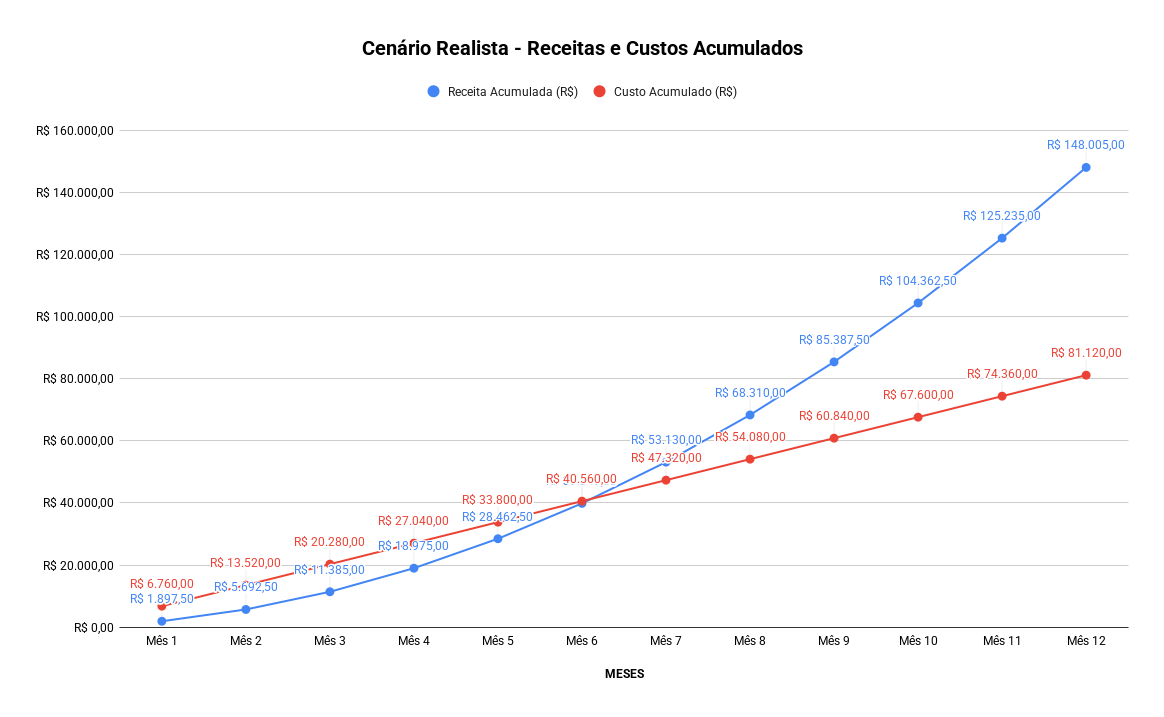
\includegraphics[width=0.9\textwidth]{cap05-viabilidade/imagens/cenario-realista.png}}
	\label{fig:cenario-realista}
	\fonte{Produzido pelos autores}
\end{figure}